\documentclass[a4paper, 10pt]{article}
\usepackage{color}
\usepackage{listings}
\usepackage{braket}
\usepackage{caption}
\usepackage{geometry}
\usepackage{graphicx}
\usepackage{amsmath}
\usepackage{ amssymb }
\usepackage{subcaption}
\usepackage{gensymb}
\usepackage{makecell}
\usepackage{listings}
\usepackage[colorlinks=true,urlcolor=blue,citecolor=blue,linkcolor=blue]{hyperref}
\usepackage{minted}


\usepackage{xcolor}

\definecolor{codegreen}{rgb}{0,0.6,0}
\definecolor{codegray}{rgb}{0.5,0.5,0.5}
\definecolor{codepurple}{rgb}{0.58,0,0.82}
\definecolor{backcolour}{rgb}{0.95,0.95,0.92}

\lstdefinestyle{mystyle}{
    backgroundcolor=\color{backcolour},   
    commentstyle=\color{codegreen},
    keywordstyle=\color{magenta},
    numberstyle=\tiny\color{codegray},
    stringstyle=\color{codepurple},
    basicstyle=\ttfamily\footnotesize,
    breakatwhitespace=false,         
    breaklines=true,                 
    captionpos=b,                    
    keepspaces=true,                 
    numbers=left,                    
    numbersep=5pt,                  
    showspaces=false,                
    showstringspaces=false,
    showtabs=false,                  
    tabsize=2
}

\lstset{style=mystyle}


\geometry{a4paper,left=25mm,right=25mm, top=2.5cm, bottom=2.5cm} 

\newcommand{\co}[1]{\texttt{#1}}


\title{Cold atoms and Qiskit}
\author{Laurin Fischer, Daniel J. Egger}
 \date{\today}


\begin{document}

\maketitle

%\tableofcontents
%\newpage

\begin{abstract}
Quantum architectures based on cold atoms have been vastly explored for the simulation of condensed matter systems in the last two decades. These rather special-purpose applications have led the quantum computing community to regard them as purely \emph{analog} quantum simulators. However, the high level of control of modern cold atomic experiments makes them candidates for quantum information processing.
Here, we investigate how such setups could be integrated in Qiskit.
\end{abstract}

\section{Cold atom specifications}

\subsection{General remarks}
In cold atom quantum simulators, well-defined quantum states are prepared using the experimental toolbox of AMO physics, including cooling techniques, optical dipole traps etc.
Here, we focus on setups where cold atoms are loaded into arrays of optical dipole traps in which a force acts on the atoms that is directly proportional to the intensity of the laser beam. 
The intensity profile of the laser therefore determines the shape of the trap.
In the case of tightly focused beams these traps are called optical tweezers.
The particles are typically cooled down enough so that they only occupy a single spatial wavefunction mode.
These modes can be populated by individual fermionic atoms obeying Pauli exclusion or, in other experiments, they may also be occupied by many bosonic atoms in a condensate.

\subsubsection{From Hamiltonians to Circuits}

After the initial state $\ket{\psi}_0$ is prepared, the experimental sequence begins (the ``quantum computation'').
This can generally be described by a many-body Hamiltonian $H_{\text{MB}}$ under which the (entire) state evolves in unitary fashion.
This Hamiltonian depends on experimental parameters $\boldsymbol{u}(t)$ that may be tunable during the evolution of the state.
The state thus evolves as 
\begin{equation}
    \ket{\psi(t)} = T \exp{ \left( - i \int_0^t H_{\text{MB}}( \boldsymbol{u}(t')) \text{d}t' \right) } \ket{\psi}_0
\end{equation}

This general language makes it difficult to get an intuition for the physics of individual operations for given parameters $\boldsymbol{u}(t)$.
One key part of the project is thus to identify a suitable description of these operations akin to the gates used in gate-based quantum computing. 

After the experimental sequence, the state is measured using imaging techniques such as fluorescence or absorption imaging.
The experimental details of this readout will vary from one experiment to another.
The specific observables that are measured in the experiments will be important for the choice of the ``computational basis''.
Ideally, the different possible measurement outcomes should correspond to a set of basis vectors of the state space. 

\subsubsection{From tweezers to wires}

A quantum circuit is a sequence of instructions that act on wires.
Here, we discuss how to map cold atom systems to these wires. The ``wires'' have several beneficial properties which are all naturally fulfilled for qubit systems:

\begin{enumerate}
    \item Each wire has a number of internal states.
    \item The segmentation into wires reflects a partition of the quantum system performing the computation.
    Ideally, the product space of the individual wires should give the Hilbert space of the entire quantum system.
    This is however only possible if the system is factorizable.
    \item The states of the wire should reflect the available measurement of the system, in such a way that a measurement of a wire (or the entire register) yields one of the internal states of the wire(s). 
\end{enumerate}

With these goals in mind, it seems natural to \textbf{assign one wire to each individual tweezer}.
The internal state of the wires are then the possible occupations of the corresponding mode, including spin degrees of freedom.
Ideally, these internal states should correspond to the different measurement outcomes of the system. 

\subsubsection{Theory-land vs. current experimental status}
It is important to exactly pin down the current experimental capabilities which will define the instructions that the experimental backends can accept.
However, for the gate description we will define in Qiskit, we aim to implement a more general model.
Moreover, in this ``theory-land'' description, larger arrays of tweezers can be defined and will enable the user to simulate these systems and explore potential applications.

In the following, we will define both the current state of the experiments and the ``theory-land'' description (see gate-based description).
Importantly, the current experiments should be describable within this extended language.


\subsection{Atomic mixtures}
    \subsubsection{Physics}
    The Jendrzejewski group works with a mixture of two bosonic atom species in the same optical dipole trap\footnote{The traps used in the Jendrzejewski group are not as deep, i.e. not as tightly focused, as tweezers. We therefore do not refer to them as tweezers.}.
    A single-mode approximation is made, meaning that only the lowest spatial mode of the trap is occupied.
    The two atomic species can be sodium (Na) and Lithium$^7$ (Li) or sodium and potassium.
    We focus on the NaLi-system for the moment.
    The most comprehensive description of this system is given in \cite{mil2020experimental}.
    Currently, the experiment runs in a single trap but can be extended to an array of trapping sites on a lattice, indexed by $n$.
    In each such trap, Bose-Einstein condensates of both atomic species are loaded, where typical atom numbers are $N_L \approx 10^4$ and $N_S \approx 10^5$.
    This number is tunable by a factor of $\approx 5$.
    
    Both species are prepared in their atomic groundstate with spin $F = 1$, and only the magnetic hyperfine states with $m_F = 0, 1$ are occupied.
    Thus, each species has two internal states which are the degrees of freedom in which the entire physics takes place.
    We associate these states with bosonic creation/annihilation operators $\hat{b}_{\alpha, n , i}$, where $\alpha \in \{L, S \}$ denotes the species (Lithium/Sodium), $n$ denotes the lattice site and $i \in \{0, 1\}$ denotes the spin.
    Thus each sodium/lithium particle is a two-state system, i.e. it can be described by a spin-$1/2$ algebra.
    The collective state of the sodium atoms on one site can conveniently be described by a large angular momentum $\hat{\vec{L}}_n$ via the \emph{Schwinger representation} by setting:
    
    \begin{equation}
        \label{eq:Schwinger_repr}
        \hat{{L}}_{z, n} = \left(  \hat{b}^\dagger_{S, n , 1}\hat{b}_{S, n , 1}  -  \hat{b}^\dagger_{S, n , 0}\hat{b}_{S, n , 0}\right)  
        \qquad 
        \hat{{L}}_{+ , n} = \hat{b}^\dagger_{S, n , 1}\hat{b}_{S, n , 0}  ,
        \qquad
        \hat{{L}}_{- , n} =  \hat{b}^\dagger_{S, n , 0}\hat{b}_{S, n , 1}    
    \end{equation}
    
     The associated $L_z$-operator for each site can thus take values of $-\frac{N_S}{2}, ..., +\frac{N_S}{2}$. This will be one of the observables in the experiment, see below. 
    
    \paragraph{System dynamics} The system dynamics consist of a permently switched on Hamiltonian $H_{\text{perm}}$ under which the state evolves.
    In addition to this, there are fast operations that can be rapidly switched on and off which includes a Hamiltonian $H_{n, n+1}$ coupling neighbouring sites. \\
    
    \noindent The physical origin of the local Hamiltonian $H_n$ are the scattering processes that take place between the particles both within their own species and with the other species.
    With an external magnetic field, the Zeeman splittings between the hyperfine levels can be tuned, which are different for both atomic species.
    This leads to an energetically favorable \emph{spin-changing interaction} in which one atom of each species switches its state.
    
    \begin{align}
        \label{eq:mixture_Hailtonian_full}
        &H_{\text{perm}} = \sum_n  H_n  \\
        &H_n = \underbrace{ \chi \hat{L}_{z,n}^2}_{\text{one-axis twisting }} 
        + \underbrace{\frac{\Delta}{2} \left( \hat{b}_{L, n , 0}^\dagger \hat{b}_{L, n , 0} - \hat{b}_{L, n , 1}^\dagger \hat{b}_{L, n , 1}\right)}_{\text{energy difference between lithium atoms}}
        + \underbrace{ \lambda \left(  \hat{b}_{L, n , 0}^\dagger \hat{L}_{-, n} \hat{b}_{L, n , 1} + \hat{b}_{L, n , 1}^\dagger \hat{L}_{+, n} \hat{b}_{L, n , 0} \right)}_{\text{spin-changing interaction}}
    \end{align}
    
    The sodium degrees of freedom only appear through their collective angular momentum operator $\hat{L}_n$ which is why we defined it in the first place.
    Let's get some intuition for the physics of the individual terms:
    
    \begin{itemize}
        \item The $\chi$-term generates dynamics on the long angular momentum vector $\hat{L}_z$. It is typically called ``one-axis twisting`` as it generates a spin-squeezed state around the x-axis, when visualized by the Husimi distribution. 
    
        \item The $\Delta$-term is proportional to the polarization of the lithium cloud. It generates a rotation around the $z$-axis of the collective angular momentum $\hat{L}$ of the lithium atoms (had we defined one). 
        
        \item The $\lambda$-term describes the spin-changing collision which is the only interaction term between the two atomic species. Each individual term coherently flips the state of both one sodium and one lithium particle. This therefore conserves the total magnetization of the system. 
        
    \end{itemize}
    
    These terms all conserve the total particle number and the total ``magnetization'' of the system.  
    Together, they form the many-body Hamiltonian under which the system evolves.
    As mentioned before, the state is at all times subject to these dynamics.
    However, they act on a rather slow timescale on the order of milliseconds.
    On a much shorter timescale, there are several other operations available that can be performed quasi-instantaneously via laser pulses:
    
    \begin{itemize}
        \item Neighbouring wells can be coupled via Raman-assisted tunneling described by the Hamiltonian
        
        \begin{equation}
        H_{n, n+1} = \underbrace{\Omega \left( \hat{b}_{L, n, 0}^\dagger  \hat{b}_{L, n+1, 1} + \hat{b}_{L, n+1, 1}^\dagger  \hat{b}_{L, n, 0} \right)}_{\text{Raman-assisted tunneling}}
        \end{equation}
        
        This terms couples lithium atoms of opposing spin state on neighbouring lattice sites. 
        
        \item The long angular momenta $\hat{L}_{\alpha, n}$ of both the sodium and the lithium atoms defined via Eq.~(\ref{eq:Schwinger_repr}) can in principle be rotated around the x, and y-axis.
        Such operations can be expressed as rotations with the $\hat{L}_x$ and the $\hat{L}_y$ angular momentum operators as the generators of a unitary transformation.
        These are defined in the canonical way from eq. \ref{eq:Schwinger_repr} as $\hat{L}_{x, n} = 1/2 (\hat{L}_{+, n}+\hat{L}_{-, n})$ and $\hat{L}_{x, n} = i/2 (\hat{L}_{-, n}-\hat{L}_{+, n})$. An $x$-rotation with a parametrization angle $\theta $ is then given as $\exp{\left(-i/2 \hat{L}_{x, n} \theta\right)} $, for example.
        Such an $x$-rotation is currently experimentally available for sodium by an optical transfer via a higher-energetic intermediate atomic state $\ket{2}$.
        A first pulse with tunable length $\tau$ takes the sodium atoms from the $\ket{\downarrow}$-state to $\ket{2}$, while a subsequent Pi-pulse takes all the atoms that made it to $\ket{2}$ back down to $\ket{\uparrow}$.
        
    \end{itemize}

    In practice, we can think of these fast operations as the actual gates that the user can use to build a circuit.
    Whenever the system is ``idle'', i.e. no such gates are applied, it will drift under the many-body Hamiltonian $H_{\text{perm}}$ for a given delay time $\tau$ that marks the time between two gates (see gate-based description).  
    
    \subsubsection{Tunability}
    
    In this system, there are some dynamics that can be tuned, and others that are permanently ``switched on''.
    Let's start our discussion with the latter. As discussed above, the many-body Hamiltonian $H_n$ within one site is permanently switched on.
    The physical origin of the parameters are discussed in sec. 4.1.2. of \cite{mil2020experimental} and briefly summarized here:
    
    \begin{itemize}
        \item $\lambda$, $\chi$ : These parameters are determined by various interaction strengths and overlap integrals of the spatial modes.
        They depend on the exact shape of the trapping potential and are thus fixed by the spatial profile of the trap beams.
        
        \item $\Delta$ : This parameter has multiple contributions, some of which are tunable:
        \begin{equation}
            \Delta = \Delta_0 + \Delta_L \frac{\hat{L}_z(t=0) }{\hat{L}} + \Delta_B \cdot B 
        \end{equation}
        The first term $\Delta_0$ is fixed by the overlap integrals of the spatial modes and the total atom numbers.
        The second term $\Delta_L$ is proportional to the initial polarization of the long sodium spin, which can be tuned over the full range from -1 to 1.
        Finally, the last term depends linearly on the applied $B$-field due to some Zeeman shifts in the level structures.
        This $B$-field is tunable within a certain range which gives some further tunability of $\Delta$.
        
        \end{itemize}
        
    The main level of control enters through the Raman-coupling of neighbouring wells and the individual spin rotations at each site, both of which can be switched on and off instantaneously. The Raman-coupling has tunable interaction strengths $\Omega$ depending on the laser intensity. The rotation angle of the spin-rotations can also be fully tuned. Although this is not yet implemented experimentally, for maximal flexibility in the gate-based description, we will assume local control over both of these operations.
    
    \subsubsection{State initialization}
        
    State initialization is discussed in \cite{mil2020experimental} and summarized here.
    Loading the micro-optical traps (MOT) takes on the order of 10s.
    After a multiple-step evaporative cooling procedure, the atoms of both species are transferred into the $m_F = 1$ ground state via a rapid adiabatic passage.
    This creates the initial state of the system.
    We associate this with the $\ket{\downarrow}$ state of the sodium atoms, thus the long sodium spins are prepared in the $\hat{L}_z/\hat{L} = -1$ state.
    
    Concerning the particle number in the system, larger atom numbers are generally preferable as this reduces the shot noise on $ \frac{\hat{N}_{S,n,1} - \hat{N}_{S,n,1}}{\hat{N}_{S,n,1} + \hat{N}_{S,n,1}}$ which is the main observable for sodium. 
    This state is not subject to any dynamics until the sodium spin $\hat{L}{z}$ is rotated away from its initial state.
    This rotation happens on a much faster timescale than the other system dynamics  and is thus called a quench.
    This sodium rotation will thus typically be the first operations in a circuit.
    We propose to give the user control over the atom number for simulator backends as this is an important degree of freedom while for the true hardware backends we will consider the atom number to be non-adjustable. 
        
    \subsubsection{Gate-based description}
        
    \paragraph{Wires}
    \label{sec:wires_mixtures}
    There are several ways to define wires for cold atom circuits.
        
    \begin{enumerate}
        \item One wire could be used to keep track of the internal states of both atomic species at a given site. \\
        \textbf{pros:} This puts all wires on an equal footing, so only a single type of wire is needed. \\
        \textbf{cons:} The different observables (lithium and sodium state occupations) can not be separated properly.
        Also, operations such as the sodium-exclusive spin rotation can not be well separated from the lithium dynamics.
            
        \item For each site, one could define two wires, where each one represents one of the two species. \\
        \textbf{pros:} Nice separation of observables and operations that may be unique to one of the atomic species. \\
        \textbf{cons:} This requires two different types of wires and therefore two different quantum registers.
        These could be two separate \texttt{QuantumRegister} instances with different names.
            
        \item If deemed unimportant, one could possibly neglect keeping track of one of the atomic species and build a circuit that gives an effective description of only one atomic species.
        Each wire would then describe the state of that species in a given site.\\
        \textbf{pros:} Only one wire type required and the description is highly simplified.\\
        \textbf{cons:} This is an option only if the degree of freedom of one species is interesting as an encoding of quantum information.
            
        \item The wires could be assigned in accordance to the observables in the experiment (See readout), i.e. for each site, assign one wire to the sodium polarization, one wire to the atom number $\hat{N}_{L, 0}$, and one to $\hat{N}_{L, 1}$.
        This approach is taken in \cite{Jendrzejewski_2020}. \\
        \textbf{pros:} Direct mapping of observables to different wire types. \\
        \textbf{cons:} Multiple wire types are required.
        Could be a bit redundant to have two wires for lithium (as the total particle number is a constant). 
    \end{enumerate}
        
    \paragraph{Gates}
    \noindent The Hamiltonian $H_n$ is always present which is a challenge for a gate-based description and will be a major issue to address when designing ``gates'' in this setup.
    \textbf{We therefor propose the following:}
    The main gates are the fast spin-rotations and Raman couplings which we will make fully tunable in the ``theory-land'' model. Between such gates, the user may set time delays $\tau$.
    This delay operation of a given duration is then simply a time evolution following the ``drift Hamiltonian'' $H_{\text{perm}}$ for a time $\tau$. 
    The local spin rotations and the Raman couplings are then conveniently described by single- and two-wire gates, respectively.
        
    As long as we are working with one lattice site, as is the current state of the experiment, it is questionable whether the system is really ``programmable'' beyond the sequence  demonstrated in \cite{mil2020scalable}.
    In this publication, the experimental sequence consists of an initial (tunable) rotation of the sodium spin after which the many-body Hamiltonian dynamics act on a state for a varied time before measurement.
    A gate-description of this experimental sequence is explored in \cite{Jendrzejewski_2020}.
    
    \subsubsection{Control setup}
        
    The entire control stack of the experiment is based on the \texttt{Labscript} software framework which offers a high level of abstraction. The central element of the user's interaction with \texttt{Labscript} is the Python \texttt{experiment.py} script that uses an abstracted description of the experiment.
    A relatively simple way to build a cold atom backend is to automatically generate the \texttt{experiment.py} script from the given list of instructions in the \texttt{QuantumCircuit} sent from Qiskit. 
        
        

    \subsubsection{Readout}
        
    For the readout, both atomic species are imaged after a Stern-Gelach separation sequence\footnote{This favors having one wire per atomic species.}.
    Here, the trap is switched off while a magnetic field gradient is applied.
    Under the subsequent time of flight, the two spin components are spatially separated.
    For each species, a laser resonant with an optical transition of the atoms is used to obtain an absorption image.
    The spatial separation of the two spin species results in two distinct clouds of atoms on the images.
    
    To assess the number of atoms in each cloud, the intensity of the region occupied by the cloud is integrated.
    As long as that intensity is linear to the total atom number, this can be calibrated to yield the total particle number of the spin for the lithium atoms. 
    This way, for both atomic species, and per trap, the number of atoms per spin state is measured, corresponding to the \textbf{observables}:
        
        \begin{itemize}
            \item The total number of sodium atoms in each spin state: $\hat{N}_{S, n, 0}$, $\hat{N}_{S, n, 1}$.
            \item The total number of lithium atoms in each spin state: $\hat{N}_{L, n, 0}$, $\hat{N}_{L, n, 1}$.
        \end{itemize}
        
        These measurements can be transformed from the total number to their sum and difference, which are more naturally suited to the ``spin-picture''.
        In this case, the sum $\hat{N}_{\alpha, n, 1} + \hat{N}_{\alpha, n, 0}$ gives the total length of the long spin, while the difference $\hat{N}_{\alpha, n, 1} - \hat{N}_{\alpha, n, 0}$ gives the $\hat{L}_z$ component.
        For example, the normalized polarization $\hat{L}_z/\hat{L}$ for sodium is given by $\frac{\hat{L}_z}{\hat{L}} = \frac{\hat{N}_{S, 1} - \hat{N}_{S, 0}}{\hat{N}_{S, 1} + \hat{N}_{S, 0}}$ .
        
        Currently, the experiment supports only one dipole trap for which $\hat{N}_{S, 0}$, $\hat{N}_{S, 1}$, $\hat{N}_{L, 0}$, and $\hat{N}_{L, 1}$ can all be measured. We assume that in a scaled-up setup these quantities can be measured for each site. We discuss how the result of these measurements is communicated to Qiskit users in Sec.~\ref{sec:qiskit_results}. 
    
    
\newpage
    
    
    \subsection{Fermionic Tweezers}
        \subsubsection{Physics}

The fermionic system consists of lattice sites formed by optical "tweezers" that can be occupied by at most one spin-up ($\uparrow$) and one spin-down ($\downarrow$) Li$^6$-particle encoded in different hyper-fine states of the atomic ground state manifold.
We further work in a lowest-band approximation, i.e. for each tweezer only the lowest-energy spatial mode is occupied.
The system is thus a near-perfect realization of \emph{local fermionic modes}.
The latest description of the setup working with up to three tweezers is given in \cite{becher2020characterizing}. 

We will denote the total amount of tweezers as $L$, and the occupations of the $i$-th site as $n_{i,\uparrow}$ and $n_{i,\downarrow}$ for the two spin states, respectively. 
As a ``computational basis'' we use the states in occupation number representation:

\begin{equation}
    \ket{\psi} = \ket{n_{1,\uparrow} \dots n_{L,\uparrow}}  \otimes \ket{n_{1,\downarrow} \dots n_{L,\downarrow} } \qquad , \qquad n_{i, \sigma} \in \{0, 1 \}
\end{equation}

This basis spans the Hilbert space of the system.
The dimension of this Hilbert space thus depends on the specific number of atoms, and not only on the register size $L$, as is the case for qubits.

The size of the Hilbert space is given by the combinatorics of placing the $N = N_\uparrow  + N_\downarrow = \sum_i n_{i,\uparrow} + \sum_i n_{i,\downarrow}$ into the available fermionic modes.
There are a total of $2L$ modes available (2 for the two spin states) in which we place $N$ particles, so total we have a Hilbert space dimension of
 \begin{equation}
    \label{eqn:hilbert_dim_number}
    \text{dim}\; \mathcal{H}\left( N \right) = {2L \choose N}
\end{equation}

If we further assume conservation of the spin of each of the particles, this further reduces to:

    \begin{equation}
        \label{eqn:hilbert_dim_spin}
        \text{dim}\; \mathcal{H} \left( N_\uparrow, N_\downarrow \right) = {L \choose N_\uparrow}  {L \choose N_\downarrow}
    \end{equation}
        
\paragraph{System dynamics}        
We will work in a model where the atoms loaded into the optical tweezer array are described by Fermi-Hubbard dynamics. 
\begin{align}
    \label{eq:fermi-hubbard-hamiltonian}
    H_{\text{FH}}(J,U,\mu) =  \underbrace{\sum_{i=1,\sigma}^{L-1} J_i (f^\dag_{i,\sigma} f_{i+1,\sigma} + \text{h.c})}_{\text{Tunneling/Hopping}} + \underbrace{U \sum_{i=1}^{L}  n_{i,\uparrow}n_{i,\downarrow}}_{\text{interaction}} + \underbrace{\sum_{i=1,\sigma}^{L} \mu_i n_{i,\sigma}}_{\text{potential offset}} 
\end{align}
The dynamics thus depend on a set of parameters $\boldsymbol{u} = \{ J, U, \mu\}$:

\begin{itemize}
    \item The parameter $J_i$ determines the strength of hopping between the site $i$ and its neighbour site $i+1$. It mainly depends on the height of the potential barrier between these two wells. This could be tuned by moving tweezers closer together or further apart, and by varying the depth of individual tweezers. These operations require delicate control on the tweezer intensities and are thus difficult to manipulate.
    
    \item The $U$ tunes the interaction of the atoms themselves.
    This is very short-range, so only particles on the same site will interact.
    Making use of a Feshbach resonance, the interaction can be tuned by an external static magnetic field.
    Depending on the sign of $U$, this can be attractive (negative $U$) or repulsive (positive $U$).
    
    \item With the aid of additional lasers, a local potential offset $\mu_i$ can be added to each site $x$. This simply raises or lowers the energy of that mode and can be tuned locally. 
    
    \end{itemize}
    
    All of the above operations are spin-conserving. In addition to these Fermi-Hubbard dynamics, there are also fast rotations of these spins available, similar to the atomic mixture system discussed above. Such rotations may be generated by Hamiltonians like:
    
\begin{equation}
    \label{eq:spin_flips}
    H_X = \sum_{i=1}^{L} \phi_i \underbrace{(f^\dag_{i,\uparrow} f_{i,\downarrow} + 
    % f^\dag_{x,\downarrow} f_{x,\uparrow})
    \text{h.c})
    }_{\text{spin flips}} \;,
    \;
    H_Z = \sum_{i=1}^{L} \phi_i \underbrace{(f^\dag_{i, \uparrow} f_{i,\uparrow} - f^\dag_{i, \downarrow} f_{i,\downarrow} )}_{\text{phase flips}} \;,
    \;
    H_Y = i \sum_{i=1}^{L} \phi_i  \underbrace{(f^\dag_{i, \downarrow} f_{i,\uparrow} - 
    \text{h.c}
    % f^\dag_{x, \uparrow} f_{x,\downarrow}
    )}_{\text{spin and phase flips}}
\end{equation}    
    
    If we think of each atom as a two-level system with $\ket{\uparrow} = \ket{0}$ and $\ket{\downarrow} = \ket{1}$, these Hamiltonians essentially generate $X$, $Y$ and $Z$-rotations on that atom. 
    These transitions can be engineered with RF pulses.
    With such RF pulses it may be possible to locally implement direct $X$, $Y$ and $Z$-rotations, which should therefore be added as gates for the simulator backend.
    These rotations happen on much faster timescales than the Fermi-Hubbard dynamics and can thus be modelled as quasi-instantaneous operations.  

\paragraph{Tunability} Crucially, the parameters $J$, $U$, $\mu$ and $\phi_i$ can in principle be tuned separately as well as be switched on and off at a given time. 
An important question is now whether these are tunable locally, i.e. for each individual tweezer, or only globally. This local control is

    \begin{itemize}
        \item very easy for $\mu$
        \item Moderately hard for $J$ and $\phi$: it would be easy to realize a single instance of random values of $J_i$, but difficult to tune them to a particular set of values (or to change them dynamically).
        \item impossible for U
    \end{itemize}

    Therefore, if we want to stay close to current experimental capabilities, it would be appropriate to work in a model with local control only on $\mu$.
    However, to fully gauge the computational potential of this system it would make sense to add locally controllable operations for $J_i$ and $\phi_i$ to the simulation backend.

    \subsubsection{Gate-based description}
    
    \paragraph{Wires}
    In the fermionic case, it seems natural to assign one wire to each tweezer, i.e. to each spatial mode of the quantized system.
    These can each have four internal states: No particles $\ket{0}$, one up-atom $\ket{\uparrow}$, one down-atom $\ket{\downarrow}$ and two atoms of each spin $\ket{\uparrow \downarrow}$.
    This description corresponds directly to the available measurements of spin- and site-resolved imaging (see Readout).
    
    The product space of these internal states is the Hilbert space that includes all possible particle numbers.
    In practice, the particle number is fixed during the state preparation and does not change throughout the experimental sequence as all operations are particle number conserving.
    For a simulator backend it would thus be more efficient to simulate the system within the subspace of a given particle number, defined by the user during the state preparation, rather than in the full state spanned by the wires.

    \paragraph{Gates}
    The basis for a gate-based description of the fermionic tweezer system is the Hamiltonian Eq.~(\ref{eq:fermi-hubbard-hamiltonian}).
    A very general, global operation that one could perform on the system would be to apply a time evolution under this Hamiltonian for some time $\tau$ with a given set of parameters $\{J, U, \mu \}$. \\ This would be a natural candidate for a general gate $U_{\text{FH}}( J, U, \mu,  \tau ) = e^{  - i H_{\text{FH}}( J, U, \mu) \tau } $.\\
    
    \noindent As a first proposal, more simple gates can be defined from this general gate in a hierarchal fashion by constraining some of the free parameters.
    This would look similar to how Qiskit implements the \texttt{U3Gate} $U_3(\theta, \phi, \lambda)$ as the most general single-qubit gate, and then defines simpler single-qubit gates by constraining the free parameters in \texttt{U3Gate}.
    One set of gates that one could define is to set all but one of the free parameters to zero, which gives the following operations:
    
    \begin{itemize}
        \item $U_{\text{hop}}(J, \tau) = U_{\text{FH}}( J, \tau, U=0, \mu=0) $
        This ``hopping''gate is a global gate (unless we assume locally tunable $J$, see above). It turns on the hopping of particles to neighbouring wells and is hence non-diagonal in the occupation number basis. This creates superposition in the occupation number basis. 
        
        \item $U_{\text{int}}(U, \tau) = U_{\text{FH}}( U, \tau, J=0, \mu=0) $
        This ``interaction''gate is always a global gate. It turns on the interaction of particles which affects only the states where two particles of opposite spin occupy the same well.
        It is thus diagonal in the occupation number basis and imprints conditional phases on the states with double occupations.
        
        \item $U_{\text{ext}}(\mu, \tau) = U_{\text{FH}}( \mu, \tau, J=0, U=0) $
        This ``external potential'' acts locally on the tweezers, and can thus be seen as a ``single-wire'' gate.
        For each index $i$ in the tweezer array, the parameter $\mu_i$ creates an external offset potential.
        This operation is also diagonal in the occupation number basis and imprints local phases. 
    \end{itemize}
    
    The local spin rotations generated by $H_x, H_y$ and $H_z$ Eq.~(\ref{eq:spin_flips}) add additional gates that break the spin-conservation symmetry.
    These can be thought of as local Pauli rotation gates on the two-level system of an individual atom.
    Finally, it will be interesting to find out how the general $U_{\text{FH}}$-gate can be used to implement various physical processes that could be described by their own gates.
    Just to name a few, such processes could be:
    
    \begin{itemize}
        \item Moving one localized particle to another tweezer. 
        \item Creating a fully delocalized superposition over all tweezers from an initially localized atom. 
        \item Performing operations on one tweezer conditional on the occupations of another tweezer 
        \item Defining transformations into other measurement bases that ideally form an informationally complete set for the readout of the state. 
    \end{itemize}
    
    Pinning down how to perform such state transformations with the available control operations will likely require substantial effort on the theoretical side but will also help build intuition for the computational capabilites of this system.
    A simulator backend will be of major interest as a central tool to play around and address these questions.
    
    A possible interface to Qiskit built on top of the existing setup would need to receive a Qiskit circuit as a set of instructions and translate/compile these high-level instructions into a timing table which can be read in by the setup.
    This is comparable to the task of compiling the Qiskit instructions into a new \texttt{experiment.py} file in the case of Labscript-controlled experiments.
    
    \subsubsection{State initialization}
    
    A typical experimental sequence that prepares the few-fermion states is discussed in \cite{becher2020characterizing}.
    As a first step in this preparation sequence, many atoms ($10^6$ are trapped in a magneto-optical trap (MOT).
    During the evaporation phase, the atomic cloud is cooled through an evaporative cooling process.
    The remaining atoms are then loaded into a tighly focussed traps, where the temperature is low enough that the fewest levels are populated with very high probability.
    In a ``spilling'' process, a potential gradient is applied which lets the atoms above a certain threshold energy escape the trap, leaving a tunable amount of atoms to remain in the trap.
    This is how the particle number can be controlled in the experiment, as further described in \cite{serwane2011deterministic}.
    From this degenerate Fermi gas, the tweezers are loaded individually with tunable atom number and spin state. 
    
    \subsubsection{Readout}
    
    Similar to the atomic mixture experiment, the state can be read out by an imaging technique that resolves the site and spin of each atom: After the experimental sequence, the potential wells of the tweezers are ramped down, which localizes each particle in one site, i.e. the state is projected onto the occupation number basis.
    The potential is then switched off, causing a time of flight expansion.
    The expanded atom cloud is then measured by collecting the resonant fluorescence atoms with an EMCCD camera through an objective with a high numerical aperture.
    The position of the atoms after time-of-flight can be related to the initial position within the tweezer array.
    The spin is determined by rapidly switching between the excitation frequencies that correspond to resonant optical transitions for both hyperfine states.
    The current experimental setup of this imaging scheme is described in \cite{bergschneider2018spin}.
    Exemplary images for two particles in a two-tweezer setup are given in \cite{bergschneider2019experimental}.
    
    Depending on the position of the collected fluorescence photons, the atoms are classified into belonging to one of the tweezers.
    This procedure seems well suited to the description of different measurement levels in Qiskit. 
    
\newpage
        
\section{Inclusion into Qiskit}
    
    \subsection{Existing functionality in Qiskit}
    
    In the following sub-sections we review the existing functionality in Qiskit that can be leverage to support cold-atom-based setups.
    
    \subsubsection{Quantum circuits, registers and wires}
    
    The central object that a user defines in Qiskit is the quantum circuit which is built internally as a list of instructions bound to registers and is implemented by the class \texttt{QuantumCircuit}.
    The instructions are a list as this grants the instructions an order. Instructions in a quantum circuit act on quantum and classical registers, which represent the qubit wires and classical bits, respectively. They are mostly unitary gates but can also include non-unitary operations like measurements or barriers.
    
    The quantum register (an instance of the \texttt{QuantumRegister} class) is a list of instances of the \texttt{Qubit} class.
    \texttt{Qubit}s have an index and register to which they belong.
    Importantly, there is no reference or implementation of a binary behavior in class \texttt{Qubit}.
    The name \emph{Qubit} may thus be a misnomer in this context. We will use the existing functionality of the \texttt{Qubit} class and will refer to them as \emph{wires}.
    
    A \texttt{QuantumCircuit} object is initialized from a list of \texttt{QuantumRegister} and \texttt{ClassicalRegister} objects. We will interpret the \texttt{QuantumRegister} as a register of abstract wires. In the fermionic case, each wire is assigend to one fermionic tweezer mode, whereas for the atomic mixtures we propose to work with two seperate \texttt{QuantumRegister}s, where the wires of one register denote the Sodium state in each tweezer and the second register describes the Lithium states.
    Instructions are implemented by the \texttt{Instruction} class (or subclasses) which requires a name, the number of wires (i.e. instances of \texttt{Qubit}) it acts upon and any parameters.
    
\subsubsection{Backends\label{sec:qiskit_backends}}
    
To run a quantum circuit in Qiskit a \texttt{backend} is chosen and the method \texttt{backend.run(...)} or \texttt{execute(qc, backend)} is called.
The results are retrieved from the backend, at the user's request, after the successful execution of the circuit.
This workflow is used for both actual hardware backends accessed through the cloud, and for simulator backends running locally. 
    
Backends communicate to Qiskit their \emph{configuration} which includes a definition of the gates that they support.
The structure of this configuration can be found in \texttt{backendconfiguration} under the module \texttt{qiskit.providers.models}.
The gates are defined by the \texttt{GateConfig} class which requires the following three parameters
\begin{itemize}
    \item name (string): the gate name as it will be referred to in QASM
    \item parameters (list of string): Variable names for the gate parameters (if any)
    \item qasm\_def (string): Definition of this gate in terms of QASM primitives $U$ and $CX$.
\end{itemize}
The following optional parameters can be given.
\begin{itemize}
    \item coupling\_map (list of lists): List of qubit groupings which are coupled by this gate.
    \item conditional (boolean): This specified gate supports conditional operations (true/false). If this is not specified, then the gate inherits the conditional property of the backend.
    \item latency\_map (list): An array of dimension len(coupling\_map) X n\_registers that specifies (1 - fast, 0 - slow) the register latency conditional operations on the gate.
    \item description (string): Description of the gate operation.
\end{itemize}
These definitions are found in \texttt{backend{\_}configuration{\_}schema.json} and in the \texttt{GateConfig} class.
The \texttt{qasm\_def} is the definition of the gate using the Quantum Assembly (QASM) language.
QASM defines gates in terms of built-in gates which are typically assumed to be the single-qubit $SU(2)$ gates and the CNOT, labeled \texttt{U} and \texttt{CNOT} respectively \cite{Cross2017}.
This is impractical for cold-atom setups as they may be non-binary.
However, QASM also allows the definition of ``Opaque'' gates:
    \begin{quote} \em
        To support gates whose physical implementation may be possible, but whose definition is unspecified, we provide an "opaque" gate declaration. [...] For example, the system may evolve under some fixed but uncharacterized drift Hamiltonian for some fixed amount of time.
    \end{quote}
We will therefore not provide a QASM definition of the cold atom gates. Rather, we will define the gates each backend accepts by specifying their name and coupling{\_}map, without giving a qasm{\_}def. What the gate does can be communicated to the user via the description string. 
    
    
\subsubsection{Result objects\label{sec:qiskit_results}}
    
Qiskit users obtain the results of their experiments through \texttt{Result} objects.
These objects are initialized from dictionaries, e.g. \texttt{Result.from\_dict(dict)}, that the backend communicates to the frontend using JSon formatted data.
This data must therefore comply to Qiskit schemas which are found in \texttt{result\_schema.json} along with examples in a subfolder.
Qiskit result objects support three measurement levels: raw, kerneld, and classified, respectively levels 0, 1, and 2.
Additionally, the data may be single-shot or averaged, see Tab.~\ref{tab:meas_formats}.
We will leverage these data formats to communicate cold atom results to users.
    
\begin{table}[htbp]
    \centering
    \begin{tabular}{c c l}\hline
            meas\_level &  meas\_return & shape \\ \hline
            0 & single & np.ndarray[shots, memory\_slots, memory\_slot\_size] \\
            0 & avg &         np.ndarray[memory\_slots, memory\_slot\_size \\
            1 & single & np.ndarray[shots, memory\_slots] \\
            1 & avg & np.ndarray[memory\_slots] \\
            2 & memory=True & list \\ \hline
    \end{tabular}
    \caption{Measurement formats in Qiskit.}
    \label{tab:meas_formats}
\end{table}
    
\subsection{Cold atom implementation in Qiskit}

The operations in a tweezer-based cold-atom experiment can be represented as a quantum circuit in which each wire is a tweezer.
Here, we will use the existing functionality in Qiskit where the instructions of the quantum circuit will act on a register of \texttt{Qubit}s which we interpret as tweezers.
As outlined above, the backend will communicate to the user which instructions it supports.
    
\subsubsection{Backends}

For both the fermion and atomic mixture hardware architectures, we propose to define two backends: Firstly, a simulator backend with instructions which correspond to those that could be implemented in future setups\footnote{Perhaps with the exception of the controllable particle number in the \texttt{prep} instruction for the mixture simulator Tab.~\ref{tab:instructions_mixtures_theory}}.
These simulators will serve as a tool to investigate the computational capabilities of such models.  
Secondly, an experimental backend that is tailored to the available operations in current experiments and allows remote control of those experiments.

Since the simulator backends describe a generalization of the current experiments, all instructions of the experimental backends, defined in Tab.~\ref{tab:instructions_mixtures_experiment}, are included in the set of accepted instructions of the simulators, defined in Tab.~\ref{tab:instructions_mixtures_theory} and~\ref{tab:instructions_fermions_theory}.
The instructions of the atomic mixture backend leverage the difference in time-scales between the fast \texttt{couple}, \texttt{rx}, \texttt{ry} instructions and the much slower \texttt{delay} instruction.

An example circuit for the atomic mixtures simulator backend (that corresponds to no particular application) is shown in Fig.~\ref{fig:NaLi_simulator_circuit}.
    
    
    \begin{table}[htbp]
        \centering
        \caption{Instructions defined for Atomic Mixtures simulator backends (``Theory-land''). The instruction column defines the purpose of the instruction. For meaning of the Name, Parameters, and Coupling map columns is discussed in Sec.~\ref{sec:qiskit_backends}.}
        \label{tab:instructions_mixtures_theory}
        \begin{tabular}{l l l c}
            % \hline\hline
            Instruction & Name & Parameters & Coupling map \\ \hline\hline
            State preparation & \texttt{prep} & \makecell[l]{System size $n$ \\ Li atom number $N_L$ \\ Na atom number $N_S$} & \makecell{Individual sites \\ both Na and Li} \\ \hline
            \makecell[l]{Evolution under \\ spin-changing collision \\ Hamiltonian} & \texttt{delay} & \makecell[l]{Evolution time $\tau$ \\ Hamiltonian param. $\Delta$} & All wires simultaneously \\  \hline
            \makecell[l]{Raman assisted \\ tunnel coupling} & \texttt{couple} & Rabi frequency $\Omega$ & Neighbouring Li sites \\ \hline
            \makecell[l]{$X$ rotation \\ on long spin} & \texttt{rx} & Rotation angle $\varphi_x$ & \makecell{Individual sites \\ both Na and Li} \\ \hline
            \makecell[l]{$Y$ rotation \\ on long spin} & \texttt{ry} & Rotation angle $\varphi_y$ & \makecell{Individual sites \\ both Na and Li} \\ \hline
            State measurement & \texttt{measure} & - & \makecell{Individual sites \\ both Na and Li} \\ \hline

        \end{tabular}
    \end{table}
    
    \begin{table}[htbp]
        \centering
        \caption{Instructions defined for Atomic Mixtures experimental backends. These instructions are a subset of those defined in Tab.~\ref{tab:instructions_mixtures_theory}.
        \label{tab:instructions_mixtures_experiment}}
        \begin{tabular}{l l l c}
            % \hline\hline
            Instruction & Name & Parameters & Coupling map \\ \hline\hline
            % State preparation & \texttt{prep} & - & - \\ \hline
            \makecell[l]{Evolution under \\ spin-changing collision \\ Hamiltonian} & \texttt{delay} & \makecell[l]{Evolution time $\tau$ \\ Hamiltonian param. $\Delta$} & All wires simultaneously \\  \hline
            \makecell[l]{$X$ rotation \\ on long spin} & \texttt{rx} & rotation angle $\varphi_x$ & Only the Na wire \\ \hline

            State measurement & \texttt{measure} & - & \makecell{Individual sites \\ both Na and Li} \\ \hline

        \end{tabular}
    \end{table}
    
    \begin{table}[htbp]
        \centering
        \caption{Instructions defined for fermionic tweezer simulator backend (``Theory-land'') }
        \label{tab:instructions_fermions_theory}
        \begin{tabular}{l l l l}
            % \hline\hline
            Instruction & Name & Parameters & Coupling map \\ \hline\hline
            % Initialize register & \texttt{init} & \makecell[l]{System size $L$} & - \\ \hline
            
            \makecell[l]{Load atoms} & \texttt{init} & \makecell[l]{Spin-state $\in \{0, \uparrow, \downarrow, \uparrow \downarrow \}$} & Individual sites \\  \hline
            
            \makecell[l]{Fermi-Hubbard \\ general evolution} & \texttt{FHGate} & \makecell[l]{ Tunnel params $J_i$ \\
            interaction $U$ \\ potentials $\mu_i$ \\ evolution time $\tau$ } & Global \\ \hline
            
            \makecell[l]{Individual \\ tunneling} & \texttt{Hop} & \makecell[l]{ Tunnel param \\ per time $\frac{J_i}{\tau}$} &  \makecell[l]{Two neighbouring \\ sites} \\ \hline
            
            \makecell[l]{Global \\ tunneling} & \texttt{HopAll} & \makecell[l]{ Tunnel param \\ per time $\frac{J}{\tau}$} &  Global \\ \hline
            
            \makecell[l]{Interaction through \\ Scattering} & \texttt{Int} & \makecell[l]{ Interaction strength \\ per time $\frac{U}{\tau}$} &  Global \\ \hline
            
            \makecell[l]{Local potential \\ offset} & \texttt{phase} & \makecell[l]{ Potential per time $\frac{\mu}{\tau}$} &  Individual sites \\ \hline
            
            \makecell[l]{Local $X$ rotation} & \texttt{Spin\_rx} & \makecell[l]{ Rotation angle $\varphi_x$} &  Individual sites \\ \hline
            
            \makecell[l]{Local $Y$ rotation} & \texttt{Spin\_ry} & \makecell[l]{ Rotation angle $\varphi_y$} &  Individual sites \\ \hline
            
            \makecell[l]{Local $Z$ rotation} & \texttt{Spin\_rz} & \makecell[l]{ Rotation angle $\varphi_z$} &  Individual sites \\ \hline
        
            State measurement & \texttt{measure} & - & - \\ \hline

        \end{tabular}
    \end{table}
    
    
        \begin{table}[htbp]
        \centering
        \caption{Instructions defined for fermionic experiment backend }
        \label{tab:instructions_fermions_experiment}
        \begin{tabular}{l l l l}
            % \hline\hline
            Instruction & Name & Parameters & Coupling map \\ \hline\hline
            
            \makecell[l]{Load atoms} & \texttt{init} & \makecell[l]{spin-state $\in \{0, \uparrow, \downarrow, \uparrow \downarrow \}$} & individual sites \\  \hline
            
            \makecell[l]{Fermi-Hubbard \\ general evolution} & \texttt{FHGate} & \makecell[l]{ tunnel params $J_i$ \\
            interaction $U$ \\ potentials $\mu_i$ \\ evolution time $\tau$ } & global \\ \hline
            
            \makecell[l]{Local potential \\ offset} & \texttt{mu} & \makecell[l]{ potential per time $\frac{\mu}{\tau}$} &  individual sites \\ \hline
            
            \makecell[l]{Local $X$ rotation} & \texttt{rx} & \makecell[l]{ rotation angle $\varphi_x$} &  global \\ \hline
        
            State measurement & \texttt{measure} & - & - \\ \hline

        \end{tabular}
    \end{table}
    
    \begin{figure}[htbp]
        \centering
        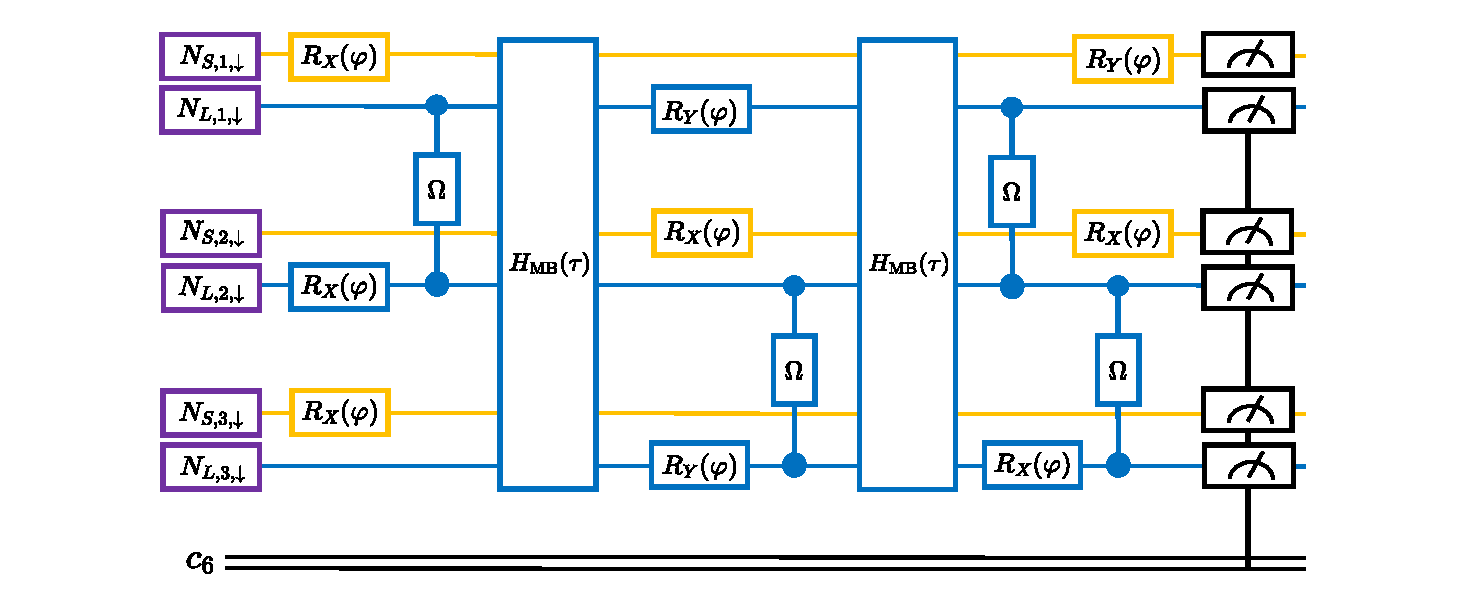
\includegraphics[width=0.7\textwidth]{figs/Na_Li_circuit.pdf}
        \caption{Example circuit build from the instructions of Tab.~\ref{tab:instructions_mixtures_theory} for the atomic mixtures simulator backend using three tweezers with one wire each per atomic species. 
        }
        \label{fig:NaLi_simulator_circuit}
    \end{figure}
    
    
    
    %\subsubsection{QuantumCircuit objects as tweezers}

\subsubsection{Result objects for cold atoms}
    
The different measurement levels defined in Qiskit, see Sec.~\ref{sec:qiskit_results}, can be leveraged to give the user control over the type of measurement data returned by the backend.
In cold atom systems, the raw measurement data is given by images taken in the experiment (absorption or fluorescence imaging).
It may thus be desirable to give the user the option to access the raw images.
This flexibility can enter through the measurement level.
For example, the level 0 could correspond to these raw images, while level 1 would return the fully processed data, i.e. atom numbers per spin state for the atomic mixtures and spin- and site-resolved occupations for the fermions.
This is summarized in tab. \ref{tab:meas_levels_cold_atoms}.
    
    % \textcolor{red}{Here we need to define what measurement levels it makes sense to return for which backends.
    % For fermions we can probably go up to measurement level 2 while for atomic mixtures we will use measurement level 1 to encode the large spin state.}
    
    \begin{table}[htbp]
    \centering
    \caption{Measurement formats in Qiskit related to the type of data returned by cold atom backends.}
    \label{tab:meas_levels_cold_atoms}
    \begin{tabular}{c l l}\hline
            meas\_level &  atomic mixtures & fermionic tweezers \\ \hline\hline
            0 & \makecell[l]{raw absorption images\\ of the atomic clouds \\ after time of flight} & - \\
            \hline
            1 & \makecell[l]{Total atom numbers \\per species, spin and site\\ extrapolated from total \\ image intensities} & \makecell[l]{Raw image of \\ fluorescence detection\\ on EMCCD camera}\\
            \hline
            2 & - & \makecell[l]{Occupation number \\of the individual tweezers \\ per spin 
            }\\
    \hline
    \end{tabular}
\end{table}
    



\section{Detailed Qiskit implementation}

Supporting cold atoms in Qiskit requires creating the required Qiskit backends, providers, and jobs classes as well as any additional required functionality. We dicuss these with special focus on the atomic mixtures system in this chapter. 

\subsection{Provider}

The Provider in Qiskit is a class that organizes and manages the access to backends. 
A typical use case of a \texttt{ColdAtomProvider} class that fulfils this task is shown below.

\begin{lstlisting}[language=Python]
from qiskit_cold_atom_provider import ColdAtomProvider

provider = ColdAtomProvider('MyToken')
backend_list = provider.backends() 
my_backend = provider.get_backend('cold_atom_mixtures')
\end{lstlisting}
The provider is initialized with an access token string, that will later be used to verify the access to the device backends when actually submitting a job to the backend. \texttt{ColdAtomProvider.backends()} returns a list of all backends that are currently supported in the provider. They each have a name and can be accessed with \texttt{ColdAtomProvider.get\_backend('backend\_name')}. When the backends are initialized, the backend server urls are queried. If the provided token is verified, the server returns the \co{configuration} dictionaries that describe all properties of a backend (more details below in sec. \ref{sec:backend_initialization}).
% \textcolor{red}{This is missing some details on what the provider does. Does it query something?}

\subsection{Backends}

Backend are the devices (hardware or simulator) that run Qiskit jobs.
To interact with backends, Qiskit provides backend classes that allow users to retrieve information about backends, send jobs to them, and retrieve results from them.
Here, we outline how to implement cold atom backends and how jobs are submitted to them.
Backends can be implemented as child classes of the \texttt{BackendV1} class in Qiskit. We aim to implement one backend for the actual experimental setup and one backend as a simulation tool for both the atomic mixtures and fermionic tweezer settings.
There are some functionalities that both experimental and simulator backends will share which is why we define another parent class to collect these. 
For example, for the atomic mixtures we define an abstract \co{AtomicMixtureBackend} class as follows.

\begin{lstlisting}[language=Python, caption = Parent class for atomic mixture backends, label = {lst:mixtures_backend_class}]
class AtomicMixtureBackend(BackendV1):
    """Abstract base class for atomic mixture backends."""

    def get_empty_circuit(self) -> QuantumCircuit:
        """Set -up an  empty  circuit  with the  right  QuantumRegisters. """
        ...

    def draw(self, qc: QuantumCircuit):
        """Modified circuit drawer to better display atomic mixture quantum  circuits."""
        ...
\end{lstlisting}
Here, we define a convenience function to initialize a circuit with the correct quantum registers, and a function to draw cold atom quantum circuits.
 The actual backend is then defined as a subclass of \co{AtomicMixtureBackend}, as shown in the following example.
\begin{lstlisting}[language=Python, caption = Example backend class, label = {lst:backend_class}]
class AtomicMixtureDevice(AtomicMixtureBackend):
    """Cold atomic mixtures backend."""

    def __init__(self, provider):
        """Initialize the backend and obtain its configuration from the URL."""
        self.url = 'backend_url'
        r = requests.get(url=self.url + '/config')
        ...

            
    @property
    def access_token(self) -> str:
        return self.provider().access_token
            
            
    def run(self, circuits: Union[QuantumCircuit, List[QuantumCircuit]],
            **kwargs) -> ColdAtomJob:
        """Send the circuits to the backend and return a cold atom job."""
        header = {
            'access_token': self.access_token,
            'meas_level': meas_level
        }

        data = circuit_to_cold_atom(circuits, shots = n_shots)

        res = requests.put(self.url, json=data, headers=header)
        res.raise_for_status()
        response = res.json()

        return ColdAtomJob(self, response['job_id'])
\end{lstlisting}

\subsubsection{Backend initialization}
\label{sec:backend_initialization}

Each backend has a unique URL assigned to it which is hard coded in the \texttt{\_\_init\_\_} method. The cold atom backend is initialized 
by making a \texttt{GET} request, using python requests, to this URL which retrieves the configuration data of the backend provided as a Json file.

The configuration is created by calling \texttt{BackendConfiguration.from\_dict(r.json())} where \texttt{r} is the result from the \texttt{GET} request.
The experimental setup must therefore return a JSon file that complies with the Qiskit schemas found in \texttt{backend\_configuration\_schema.json}.
The configuration schemas comprise all relevant information needed for working with the backend.
As an instructive example for the structure of this Json file, we show below what a configuration could look like for the atomic mixture experimental backend.

\begin{lstlisting}[language=Python, caption = Example backend configuration that the remote backend server must return when the Qiskit user runs \texttt{provider.get\_backend('atomic\_mixture')}., label={lst:backend_configuration}]
{'backend_name': 'atomic_mixtures',
 'backend_version': '0.0.1',
 'n_qubits': 2,     # number of wires
 'atomic_species': ['Na', 'Li'] , 
 'basis_gates': ['delay', 'rx'],
 'gates': [
    {'name': 'delay',
     'parameters': ['tau', 'delta'],
     'qasm_def': 'gate delay(tau, delta) {}',
     'coupling_map': [[0, 1]],
     'description': 'evolution under SCC Hamiltonian for time tau'},
    {'name': 'rx',
     'parameters': ['theta'],
     'qasm_def': 'gate rx(theta) {}',
     'coupling_map': [[0]],
     'description': 'Rotation of the sodium spin'}],
 'supported_instructions': ['delay', 'rx', 'measure', 'barrier'],
 'local': False,            # backend is local or remote (as seen from user)
 'simulator': False,        # backend is a simulator
 'conditional': False,      # backend supports conditional operations
 'open_pulse': False,       # backend supports open pulse
 'memory': True,            # backend supports memory
 'max_shots': 60,
 'coupling_map': [[0, 1]],
 'max_experiments': 3,
 'description': 'Setup of an atomic mixtures experiment with one trapping site and two atomic species, namely Na and Li.',
 'url': 'http://url_of_the_remote_server',      
 'credits_required': False,
 'online_date': datetime.pyi = hopefully soon,
 'display_name': str = None}\end{lstlisting}
 
\noindent We now discuss some of the entries in this JSon file in more detail.
\begin{itemize}
    \item \texttt{'n\_qubits'} gives the maximum amount of wires (which are \co{Qubit} objects in Qiskit, hence the name) that an incoming circuit can have. In this case, we describe the experiment with one wire per atomic species, so \co{n\_qubits = 2}. 
    
    \item \co{'basis\_gates'} is a list of the supported instructions. These are defined via the \co{GateConfig} class whose sepcifications are given as a dictionary under the key \co{'gates'}. Note that in the \co{qasm\_def}, the actual specification \co{\{\}} remains empty. The \co{'coupling\_map'} defines on which wires (\co{Qubit}s) these gates can be executed. As the \co{rx} gate can only be applied to the sodium wire, its \co{coupling\_map} is \co{[[0]]}.
    
    \item \co{'supported\_instructions'} is a list of the names of all instructions that can be applied to a circuit to be run on this backend. This includes the names of all the gates but also non-unitary instructions such as measurements and barriers. 
    
    \item For now we set \co{'open\_pulse'} to \co{False}. This means that the backend will not accept \co{PulseJob}s which are defined in \co{OpenPulse}. This functionality may be added later to give users pulse-level access to the hardware. 
    
    \item The maximum amount of shots for a single quantum circuit in one job is given by \co{'max\_shots'}. A job can consist of multiple quantum circuits that a user wants to execute. The maximum number of different circuits per job is thus bounded by \co{'max\_experiments'}. 
    
    \item The \co{'url'} of the backend gives the network address of the remote server to which the user communicates their job requests. 
    
    \item Some backends may wish to manage how many jobs a user can run. This can be done by requesting that users have sufficient credits to run jobs. If credits are required then the \co{'credits\_required'} keyword is set to \co{True}. 

\end{itemize}

The exact specifications of what this backend configuration file needs to look like is detailed in Qiskits \co{QasmBackendConfiguration} class. There are also some additional, optional keyword arguments not specified in the example above. After initialization, the backend configuration can be accessed via \co{my\_backend.configuration().to\_dict()}. 

\subsubsection{Cold atom gate libraries}

All gates that we will define in Qiskit for the cold atom setups will be collected in a \co{ColdAtom.circuit.} \co{library} file from which they can be imported directly, akin to the \co{qiskit.circuit.library} for conventional quantum gates. 
They are defined as child classes of qiskit's \co{Gate} base class:

\begin{lstlisting}[language=Python, caption = definition of a cold atom gate in qiskit, label={lst:gate_definition}]
class ColdAtomRXGate(Gate):
    """Rotation of the collective spin of a cold atomic BEC around the x-axis"""

    def __init__(self, theta, label=None):
        """Create new RX gate."""
        super().__init__('rx', 1, [theta], label=label)

    def inverse(self):
        """Return inverted RX gate"""
        return ColdAtomRXGate(-self.params[0])
\end{lstlisting}

It is crucial to give the same name to this gate (here \co{'rx'}) as is given in the backend configuration in Lst.~\ref{lst:backend_configuration}. Other versions of this gate, like an inverse can also be directly implemented in this gate class. 

\subsubsection{Running cold atom circuits on the backends}

\paragraph{Creating a circuit} Users can leverage the circuit library to create quantum circuits tailored to cold atom backends.
In Lst.~\ref{lst:circuit_definition} we exemplify this for the NaLi backend with a rotation of the Sodium atoms followed by a time-evolution under the drift Hamiltonian.

\begin{lstlisting}[language=Python, caption = example for defining a quantum circuit, label = {lst:circuit_definition}]
from ColdAtom.circuit.library import ColdAtomRXGate, ColdAtomSCCdrift

qc = backend.get_empty_circuit()

qc.append(ColdAtomRXGate(theta=0.7), qargs=[na_reg[0]])
qc.append(ColdAtomSCCdrift(tau=20) , qargs=[na_reg[0], li_reg[0]])
qc.measure([0,1], qc.cregs[0])
\end{lstlisting}

As mentioned in sec. \ref{sec:wires_mixtures}, for the atomic mixture experiment, we propose to use two \co{QuantumRegister}s for the two species, called \co{na\_reg} and \co{li\_reg} here.
They are pre-defined in the \co{get\_empty\_circuit} method of the base \co{AtomicMixtureBackend} class, so that the user will know what kind of circuit structure the backend expects. 
Here, we import the sodium $x$-spin rotation and the SCC Hamiltonian gate.
We then add these gates to the wires with the \co{append} method of \co{QuantumCircuit}, assigning the desired values for the free parameters in the gates, \co{theta} and \co{tau}.
Finally, a measurement is added between both wires and the classical register (also pre-defined by \co{get\_empty\_circuit}).

\paragraph{Running the circuit}
\noindent This circuit is now ready to be sent to the backend. The syntax for this is:
\begin{lstlisting}[language=Python]
job = my_backend.run(List[QuantumCircuit], **kwargs)
\end{lstlisting}
The backends each have a method called \co{run}, which accepts a list of quantum circuits. The additional \co{kwargs} comprise all further options, like shot numbers, measurement level etc. 
The \co{run} method is the central point of communication between the user and the backend so let's examine this part in detail (see lines 16-30 in lis. \ref{lst:backend_class}).

\co{run} converts the circuit into a Json serializable \co{dict} and sends it to the backend url via a \co{PUT} request. Additional parameters are sent along in the \co{header} dict.
The circuits are converted into the \co{dict} by the hard-coded \co{circuit\_to\_cold\_atom()} function.
This \co{dict} has the structure shown in List~\ref{lst:circuit_json}.
Each circuit has a unique identifier \co{experiment\_id}.
Each circuit is then specified by its \co{data} where \co{inst\_name} is a reserved name and takes on the value of one of the basis instructions supported by the hardware as communicated by its configuration file.
\co{wires} indicates the wires in the circuit that the instruction is applied to.
\co{wires} therefore indicates the trapping site and atomic species to which the instruction is applied.
Finally, \co{params} is the list of parameter values, e.g. a rotation angle, that the instruction takes.
\co{shots} defines the number of times the circuit is repeated.

\begin{lstlisting}[language=Python, caption = Incoming circuit data received by the backend as a Json dictionary., label = {lst:circuit_json}]
{
    experiment_id(str): {
        'instructions': [
            (inst_name(str), wires(List[int]), params(List[float])),
        ], 
        'shots': int, 
        'num_wires': int
    }
 }
\end{lstlisting}
For example, the json that would be created for the circuit above looks like:
\begin{lstlisting}[language=Python, caption = Example of incoming circuit data received by the NaLi device backend as a Json file. The instructions in data show that this circuit is to be run with one trapping site. An \co{rx} rotation with angle 0.7 radians is applied to the Na atoms followed by a 20 ms delay. Finally the Na atom is measured., label = {lst:circuit_json_example}]
{
    'experiment_0': {
        'instructions': [
            ('rx', [0], [0.7]), 
            ('delay', [0, 1], [20]), 
            ('measure', [0], []),
            ('measure', [1], [])
        ], 
        'num_wires': 2,
        'shots': 10
    }
 }
\end{lstlisting}
The \co{PUT} method of the web API will then handle this request and process it further.  In the case of the atomic mixtures backend, this will include the following steps:
\begin{itemize}
    \item Verification of the provided \co{access\_token}.
    \item Assigning a unique job ID and placing the job in a queue
    \item Processing the circuit. This includes validating\footnote{This step should determine if the input data corresponds to the outlined format and that all parameter values, including wire numbers, are within acceptable ranges.} the input JSon data and converting it into a suitable \co{experiment.py} file for the control setup and running the experiment. 
\end{itemize}
The \co{response} of this \co{PUT} request sent is sent back to the user as a Json that includes the \co{job\_id}.
This unique identification number is created by the backend for each submitted \co{data} file.
The \co{job\_id} is subsequently used to define a \co{Job} object which is the central object in Qiskit that is created to manage the handling of the submitted task. 

\subsection{Jobs}
A Job has a unique Id and is what allows the user to recover results from a backend.
Cold atom jobs can be supported with a \co{ColdAtomJobs} class  that inherits from Qiskits \co{JobV1} class. The class definition will look like this: 

\begin{minipage}{\linewidth}
\begin{lstlisting}[language=Python, caption = Job class that encapsulates information about the job submitted to the backend, label = {lst:job_class}]
class ColdAtomJob(JobV1):

    def __init__(self, backend: Backend, job_id: str):
        super().__init__(backend, job_id)


    def result(self, wait: float = 5.0) -> Result:
        """Retrieve a result from the backend."""
        
        while True:

            params = {'job_id': self._job_id, 'access_token': self._backend.access_token}
            result_dict = requests.get(self._backend.url, params=params).json()

            if result['status'] == 'finished':
                break
                
            time.sleep(wait)
                
        return Result.from_dict(result_dict)


    def status(self) -> JobStatus:
        """
        Query the backend  to get the status of the job based on 
        HTTP status codes.
        """
        result = requests.put(self._backend.url + '/status',
                              json={'job_id': self._job_id,
                                    'access_token': self._backend.access_token})

        status = result.status_code
        ...
        
    def cancel(self):
        """Send a cancellation request to the backend."""
        pass
\end{lstlisting}
\end{minipage}

A Job object is defined from the chosen backend and its unique \co{job\_id}. This is how the \co{backend.run()} method initializes the Job. Any \co{Job} class in Qiskit then comes with two important methods:

\begin{itemize}
    \item With the \co{result} method, the user can contact the backend and ask to retrieve the results from the execution of the circuit(s) on the backend with a \co{GET} request on the backend's URL.
    The method repeatedly queries the backend (every \co{wait} seconds), providing the correct \co{job\_id} that was originally assigned to the job when calling \co{backend.run()}.
    Internally, the backend server then checks whether the task with the given \co{job\_id} has finished, in which case
    a Json dictionary is returned to the user which includes all information about the experimental results and the key-value pair \co{'status': 'finished'}.
    On the user side, this is converted into a Qiskit \co{Result} object.
    We'll address the required formatting of the \co{result\_dict} for this step in more detail in sec. \ref{sec:design_results}.
    If the key-value pair \co{'status': 'finished'} is not present in the returned Json then the job is considered not finished.
    If the key-value pair \co{'status': 'error'} is  present in the returned Json then the job has failed.
    
    \item With the \co{status} method, the used can check the status of the submitted job. 
    The backend is contacted once through a \co{PUT} request where the user is again identified by his \co{access\_token} and \co{job\_id}.
    The HTTP \co{status\_code} of the request's answer is converted into a Qiskit \co{JobStatus} object and returned to the user.
    The Qiskit backend will handle the HTTP status codes following Tab.~\ref{tab:job_status}.
    
    \item A \co{cancel} method allows users to abort a previously issued job. 
\end{itemize}

\begin{table}[]
    \centering
    \begin{tabular}{l l l} \hline
         code & Qiskit Status & Meaning \\ \hline\hline
         100 & JobStatus.RUNNING & The Qiskit Job is running. \\
         200 & JobStatus.DONE & The job is finished and the user can query his results.\\
         201-202 & JobStatus.INITIALIZING & \\
         Everything else & JobStatus.ERROR & Something went wrong \\ \hline
    \end{tabular}
    \caption{How the Qiskit backend handles HTTP status codes when doing \co{job.status()}. Extra HTTP status codes could be added if more granularity is needed.}
    \label{tab:job_status}
\end{table}


\subsection{Results} \label{sec:design_results}

To describe job results Qiskit provides the \co{Result} class which we use without further modifications.
The Json dictionary that is returned when a user queries the backend for the result of his job can be turned into a \co{qiskit.Result} object via the \co{Result.from\_dict()} method.
A minimal configuration of the data returned by the backend is shown in Lst.~\ref{lst:minimal_res_dict}:

\begin{lstlisting}[language=Python, caption = configuration of result dictionary returned by the backend as a Json dictionary, label = {lst:minimal_res_dict}]
{
    "backend_name": str,
    "backend_version": str,
    "job_id": str,
    "qobj_id": str,
    "success": bool,
    "header": dict,  # must be JSon serializable
    "results": list[
        {   
            "header": dict,  # must be JSon serializable
            "shots": int,
            "success": bool,
            "meas_return": str,
            "meas_level": int,  # most likely always 1 or perhaps 0
            "data": {
                "counts": dict,  # must be JSon serializable
                "memory": list 
            }
        }
    ]
}
\end{lstlisting}

The actual information about the results of the (possibly multiple) \co{QuantumCircuit}s is given as dictionaries themselves, which are provided as a list under the \co{"results"} key. Each element in this list corresponds to one experiment (i.e. \co{QuantumCircuit}).
For each individual circuit, there are two main ways the results are stored.
The default way is to store the measurement results as a dictionary under the key \co{"counts"}.
This dictionary groups the different shots by their different measurement outcomes and simply counts the occurrences of each outcome.
For example for a two qubit circuit with 10 shots this may look like:
\begin{lstlisting}
"counts": {"00": 3, "01": 1, "10": 4, "11": 2}
\end{lstlisting}
This count dictionary can be accessed via the \co{Result.get\_counts()} method.
For the atomic mixtures we have many more degrees of freedom in the observables, so this way of communicating the result may be infeasible.

If the backend supports memory, i.e. \co{"memory":True} in the backend \co{config}, then the individual measurement outcomes of each shot are returned as a list under the \co{"memory"} key and can be accessed through \co{Result.get\_memory}.
This is more appropriate for the cold atom experiments.
The \co{get\_memory} function implemented in Qiskit \co{Result} can return the memory for a specific experiment if given an index or experiment name as argument.
The format of the list returned by memory depends on the \co{meas\_return} type. If single-shots are returned the dimension of the memory is the number of shots times the number of \emph{memory slots}.
Each wire has one memory slot.
Each entry in the memory is specified as a list of two numbers.
For the cold atom backend the first number will represent the number of atoms in the spin-up state while the second number will be the number of atoms in the spin down state.
When \co{result.get\_memory()} is called these two numbers are returned as a single complex number. This formatting is a result of the IQ plane description of superconducting qubits.
An example of a result is shown in Lst.~\ref{lst:minimal_res_example}.
If averaged results are returned the memory has one dimension less as the shots are averaged, see the example in Lst.~\ref{lst:minimal_res_example_avg}.

\begin{minipage}{\linewidth}
\begin{lstlisting}[language=Python, caption = Example of a result returned by the NaLi device backend as a Json dictionary. The result has one experiment (namely \co{experiment\_0} which matches the name in Lst.~\ref{lst:circuit_json_example}) with three shots and two wires (one for Na and one for Li). In the first shot there are 90012 Na atoms in the spin-up state and 9988 in the spin-down state., label = {lst:minimal_res_example}]
{
    "backend_name": "atomic_mixtures_device",
    "backend_version": "0.0.1",
    "job_id": "dae51c52-5caa-11eb-b265-080027f905c2",
    "qobj_id": None,
    "success": True,
    "header": {},
    "results": list[
        {   
            "header": {"name": "experiment_0", "extra metadata": "text"},
            "shots": 3,
            "success": True,
            "meas_return": "single",
            "meas_level": 1,
            "data": {      # slot 1 (Na)      # slot 2 (Li)
                "memory": [[[90012.,  9988.], [5100., 4900.]],  # Shot 1
                           [[89900., 10100.], [5000., 5000.]],  # Shot 2
                           [[90000., 10000.], [5050., 4950.]]]  # Shot 3
            }
        }
    ]
}
\end{lstlisting}
\end{minipage}


\begin{minipage}{\linewidth}
\begin{lstlisting}[language=Python, caption = Part of the data in Lst.~\ref{lst:minimal_res_example} modified to the case where average results are returned to the user., label = {lst:minimal_res_example_avg}]
            "shots": 3,
            "meas_return": "avg",
            "meas_level": 1,
            "data": {      # slot 1 (Na)      # slot 2 (Li)
                "memory": [[89971.,  10029.], [5050., 4950]]  # Average of three shots
            }
\end{lstlisting}
\end{minipage}

The \co{meas\_level} and \co{meas\_return} (optional) keys indicate what kind of data is being returned, as classified in Tab.~\ref{tab:meas_formats}. Finally, depending on the backend, instead of \co{counts} or \co{memory}, the dictionary of the \co{"data"} key can also include \co{statevector}, \co{unitary} or \co{snapshot} keys, which add further flexibility to the datatypes that can be returned in a result object.

\begin{figure}
    \centering
    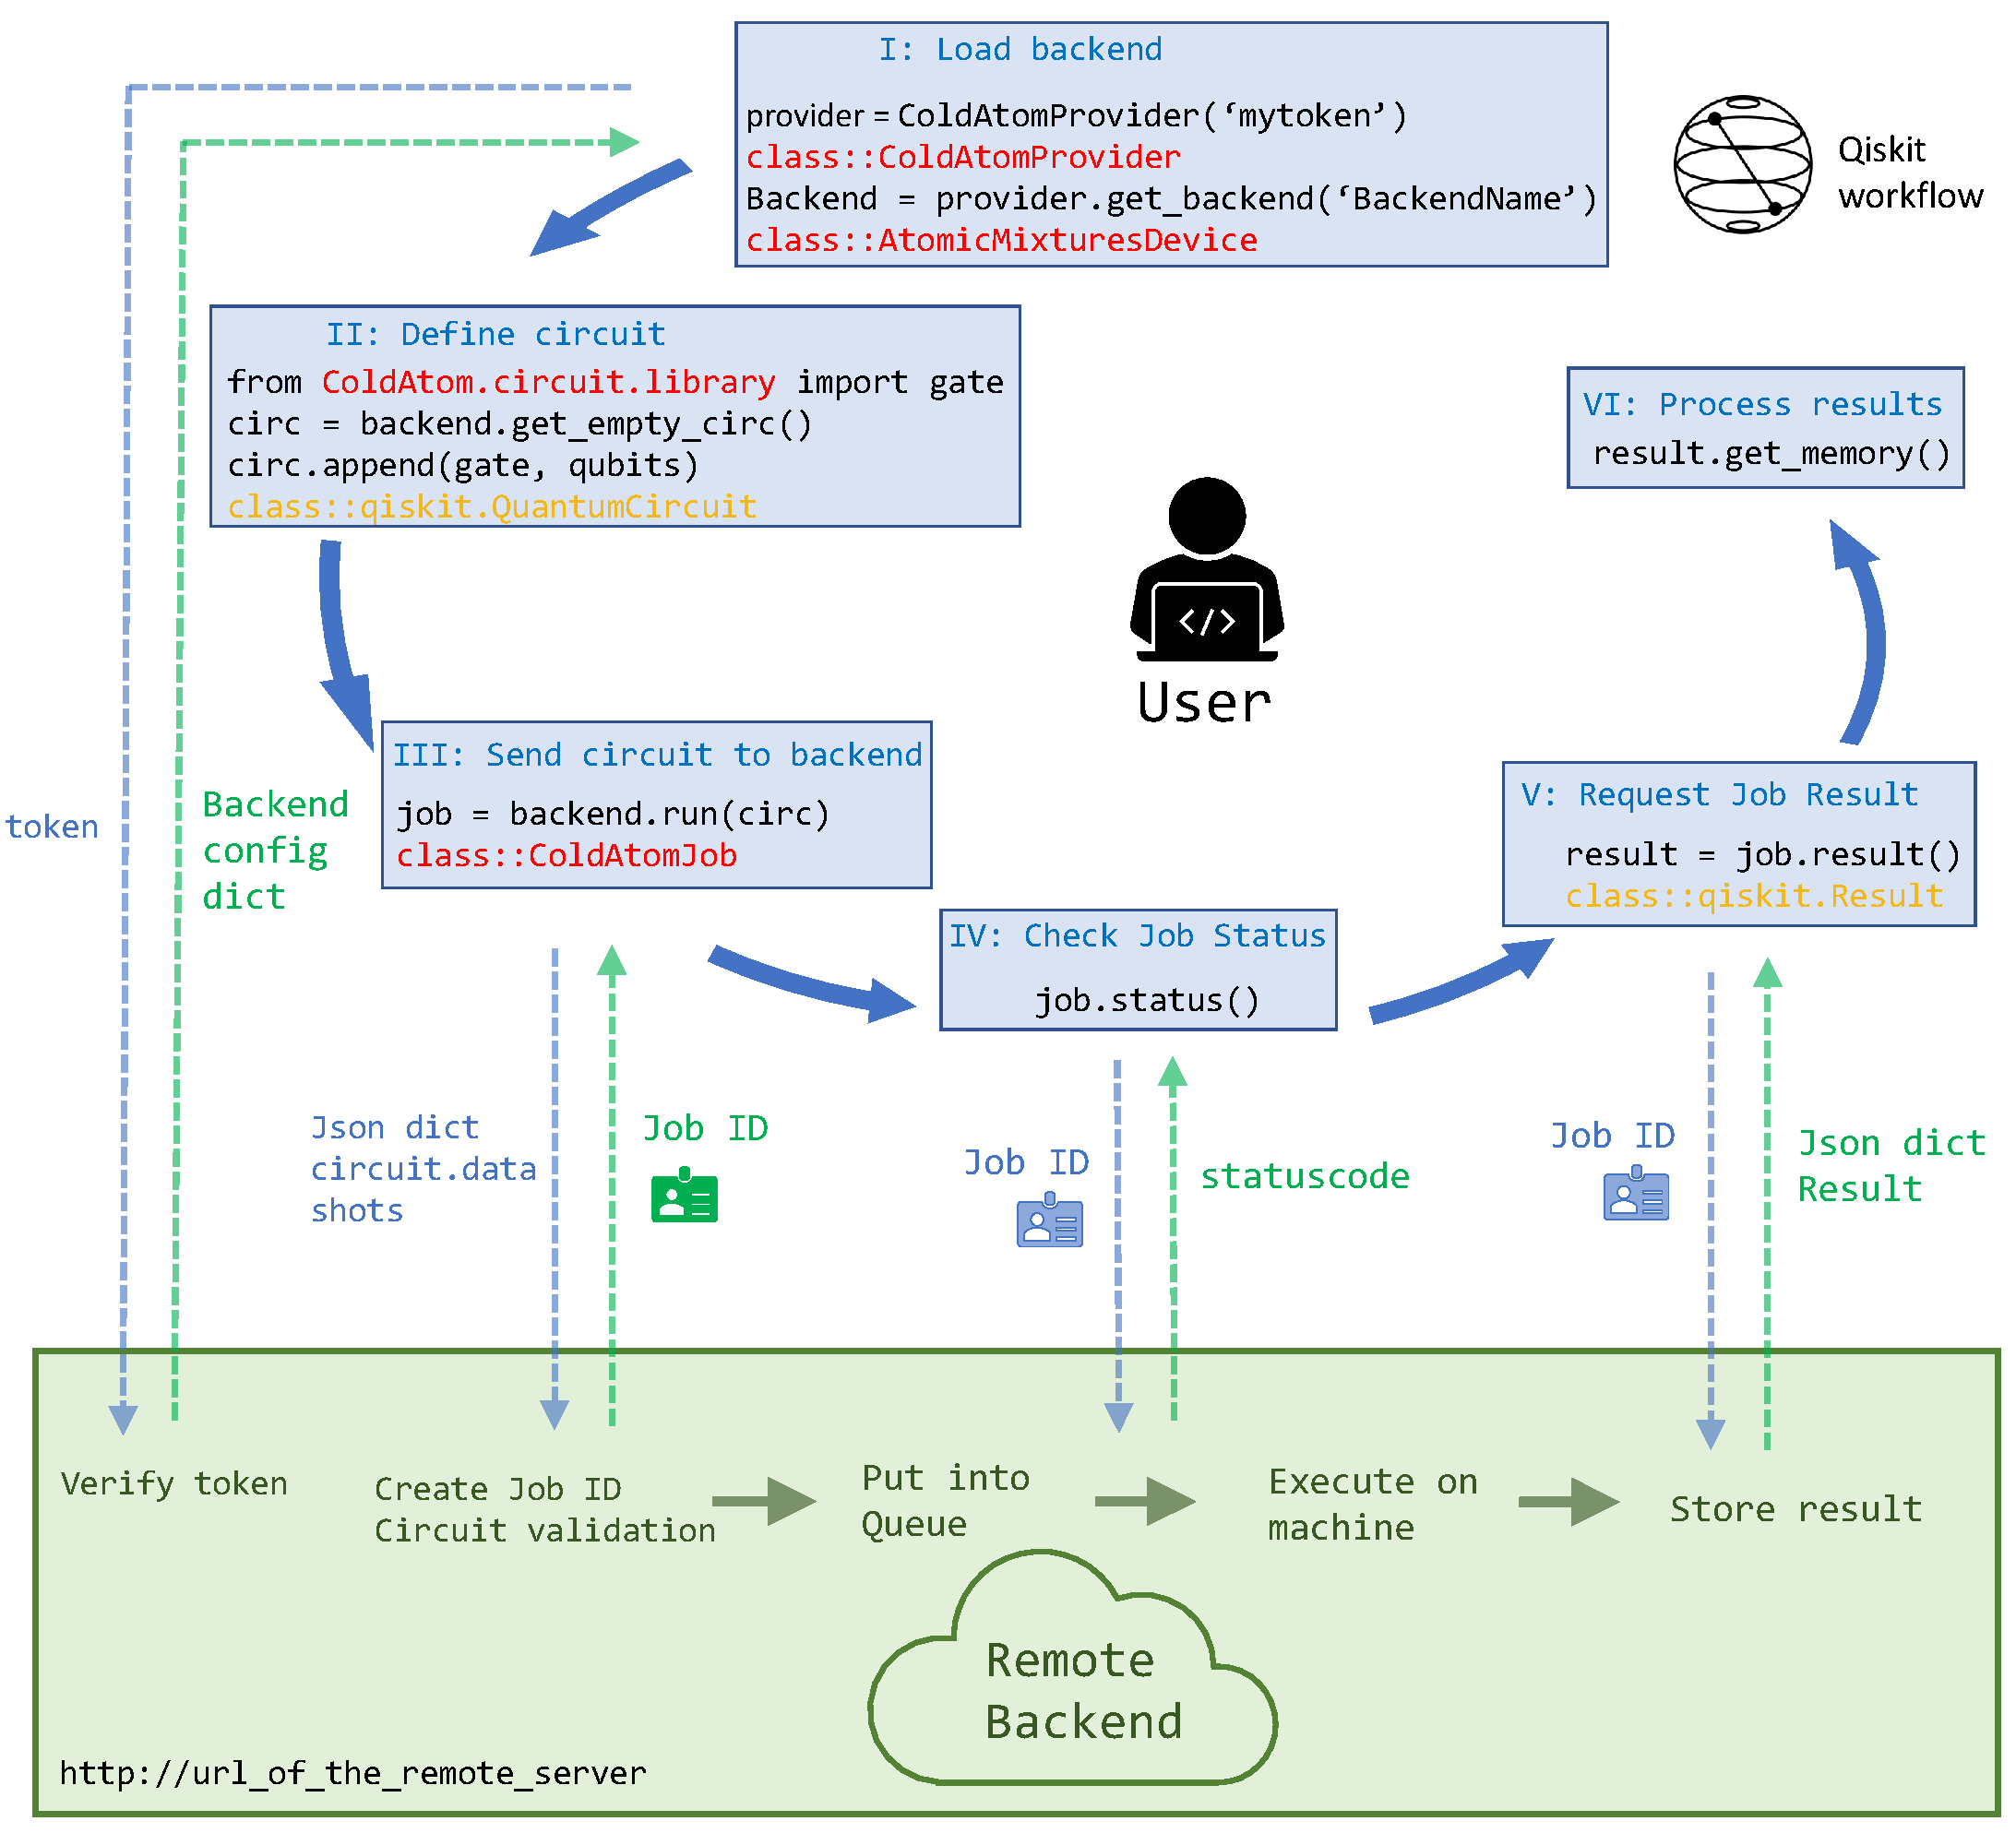
\includegraphics[width=0.99\textwidth]{figs/workflow_diagram.pdf}
    \caption{Schematic of the workflow to include a cold atom remote backend into Qiskit.
    Red parts in the pseudocode highlight new classes and functionalities we need to implement while yellow shows where we can use existing classes from Qiskit without further modification.
    Blue dashed arrows indicate all points where requests are sent form the user to the backend url, while green dashed arrows symbolise the response to those requests. }
    \label{fig:workflow_diagram}
\end{figure}

\subsection{Summary}

In Fig.~\ref{fig:workflow_diagram}, we give an overview of how the different Qiskit components discussed in this chapter interact for the execution of circuits on a cold atom experimental backend.
We also schematically show the relevant steps happening on the remote backend which will need to be implemented.
These include: token management, receiving, validating and queuing the received circuits, queue management, connecting to the control setup, storing the results, providing the results upon user requests.

\subsection{Steps to be done on the remote backend}

Here we summarize the steps that need to be addressed on the remote backend to enable remote control of the exepriment as a Qiskit backend.
Firstly, a server is needed as the central url on which the backend is hosted.
As shown in fig. \ref{fig:workflow_diagram}, the user send all of his request to this central url. 

\subsection{Token Management}
For a remote backend, the user verification in Qiskit can be handled through a token management system.
In order to give access to a user, a token has to be issued, which the user has to supply in order to load the configuration of the backend.

\subsection{Receiving the circuits}
The central communication between the experimental backend and the user happens through the exchange of Json files.
This is first and foremost the incoming Json file of the quantum circuits (see Lst.~\ref{lst:circuit_json_example} for an example) that the user sends to the backend when initializing his job.
Processing this on the backend includes the following steps:
\begin{itemize}
    \item First of all, the circuit needs to be validated to match the requirements of the backends.
    This includes making sure the register and the gates match the backend configuration and checking that all free gate parameters are within the experimental capabilities. 
    \item If the circuits are successfully validated, the backend creates a Job-Id which is returned to the user for future references like checking for status and results. 
    \item The job will then need to be placed in a queue.
\end{itemize}
\subsection{Queue management}
The management of the queue is left to the setup to implement as needed. 

\subsection{Connecting to Labscript}
For an experimental control stack built within the \co{Labscript} framework, connecting to the experimental control could be relatively easy.
This would require a routine that translates the Json files of the incoming quantum circuits into the appropriate \co{experiment.py} file.
For each instruction that the backend supports (gates, state preparation and measurements), this routine needs to translate these instructions into the more complicated experimental commands in \co{Labscript}. 

\subsection{Result storage} 
After the user's circuits are executed on the machine, the results need to be stored locally on the backend server.
It is the user that will request these results.
To return them, they need to cast into the required Json format shown in Lis.~\ref{lst:minimal_res_dict}.
This will require a second routine that translates between labscript's data storage format and this Json schema. 

\nocite{*}
\bibliography{refs}
\bibliographystyle{plain}

\end{document}
